\chapter{Project Requirements}
This chapter describes the functional and non-functional requirements of the PawPal pet care mobile application. The requirements are gathered through use case analysis, stakeholder, and competitive analysis of existing pet care solutions.

\section{Use Case Analysis}
PawPal is an interactive end-user mobile application, making use case modeling the most appropriate requirement gathering technique. The following use cases represent the core functionalities across all eight modules of the system.

\subsection{High-Level Use Cases Overview}

The PawPal system supports twelve primary use cases that span across all eight modules, providing comprehensive pet care functionality:

\begin{enumerate}
    \item \textbf{User Registration and Authentication} - New users create accounts and existing users authenticate to access system features
    \item \textbf{Pet Breed Identification} - AI-powered breed recognition from uploaded pet photos with personalized care recommendations
    \item \textbf{AI Chatbot Consultation} - 24/7 virtual veterinary assistant providing instant health guidance and emergency support
    \item \textbf{Pet Profile Management} - Comprehensive digital pet profiles with health records, vaccination tracking, and journal maintenance
    \item \textbf{Marketplace Commerce} - End-to-end e-commerce for pet products including browsing
    \item \textbf{Veterinary Services} - Appointment booking, clinic discovery, and consultation management with healthcare providers
    \item \textbf{Caregiver Services} - Professional pet care service booking with real-time tracking and service completion verification
    \item \textbf{Community Participation} - Social networking features including posts, groups, events, and content sharing
    \item \textbf{Lost Pet Alert System} - Emergency alert broadcasting with community engagement and GPS-based notifications

    \item \textbf{Payment Processing} - Secure payment gateways using cryptocurrency transactions
    \item \textbf{System Administration} - Platform management including  dispute resolution, blocking users, handling payment errors 
\end{enumerate}

These high-level use cases encompass all stakeholder interactions including Pet Owners, Veterinarians, Caregivers, Marketplace Sellers, and System Administrators, ensuring comprehensive coverage of the PawPal ecosystem.

\subsection{Fully Dressed Use Cases}

The following detailed use cases follow the comprehensive use case template, providing complete specifications for each core system functionality.

\textbf{UC-0: User Registration and Authentication}

\textbf{Use Case ID:} UC-00

\textbf{Use Case Name:} User Account Registration and Login

\textbf{Scope:} PawPal Pet Care System

\textbf{Level:} User-goal level

\textbf{Primary Actor:} New User / Existing User

\textbf{Stakeholders and Interests:}
\begin{itemize}
    \item New Users: Want simple, secure account creation process
    \item Existing Users: Need reliable, fast authentication
    \item System Administrators: Require secure user management with fraud prevention
    \item All Stakeholders: Need data privacy and security compliance
\end{itemize}

\textbf{Preconditions:} User has mobile device with internet connection and valid email address

\textbf{Postconditions (Success Guarantees):} User account is created or authenticated, session is established, and user can access system features

\textbf{Minimal Guarantees (Failure Guarantees):} Failed attempts are logged, account security is maintained, and user receives clear error messages

\textbf{Trigger:} User opens PawPal application for first time or selects login option

\textbf{Main Success Scenario:}
\begin{enumerate}
    \item User opens PawPal application
    \item System displays registration/login options
    \item User selects "Create New Account" or "Login"
    \item For Registration: User enters email, password, confirms password, accepts terms
    \item For Login: User enters email and password
    \item System validates credentials and checks security requirements
    \item System sends email verification (registration) or validates session (login)
    \item User confirms email verification if registering
    \item System creates secure session with JWT token
    \item User gains access to main dashboard and system features
\end{enumerate}

\textbf{Extensions (Alternate Flows):}
\begin{itemize}
    \item 4a. Invalid email format: System displays error and requests valid email
    \item 4b. Weak password: System provides password strength requirements
    \item 4c. Email already exists: System suggests login or password reset
    \item 6a. Login credentials invalid: System increments failed attempt counter
    \item 6b. Account locked due to failed attempts: System requires password reset
    \item 7a. Email verification fails: System resends verification email
    \item 8a. Email verification expires: System allows new verification request
\end{itemize}

\textbf{Special Requirements:}
\begin{itemize}
    \item Security: bcrypt password hashing with minimum cost factor 12
    \item Performance: Authentication within 5 seconds

\end{itemize}

\textbf{Technology and Data Variations:}
\begin{itemize}
    \item Authentication: JWT tokens with 24-hour expiration
    \item Password reset: Email-based reset with secure token
    \item Social login: Future integration with Google/Apple authentication
    \item Multi-factor authentication: SMS or app-based 2FA option
\end{itemize}

\textbf{UC-1: Identify Pet Breed}

\textbf{Use Case ID:} UC-01

\textbf{Use Case Name:} AI-Powered Pet Breed Identification

\textbf{Scope:} PawPal Pet Care System

\textbf{Level:} User-goal level

\textbf{Primary Actor:} Pet Owner

\textbf{Stakeholders and Interests:}
\begin{itemize}
    \item Pet Owner: Wants accurate breed identification to understand pet characteristics and care requirements
    \item AI/ML System: Needs high-quality images for accurate CNN model inference
    \item Veterinarians: Benefit from accurate breed information for health recommendations
\end{itemize}

\textbf{Preconditions:} User is logged in, has camera permissions enabled, and pet image is available

\textbf{Postconditions (Success Guarantees):} Pet breed is accurately identified, stored in database, linked to pet profile, and care recommendations are provided

\textbf{Minimal Guarantees (Failure Guarantees):} User receives error notification, failed attempt is logged, and user can retry with different image

\textbf{Trigger:} User navigates to Pet Identification module and initiates breed detection

\textbf{Main Success Scenario:}
\begin{enumerate}
    \item User navigates to Pet Identification module
    \item User captures new photo or uploads existing photo of their pet
    \item System validates image quality and format (JPEG/PNG, max 10MB)
    \item System processes image through CNN model
    \item System displays breed identification with confidence score (0-100\%)
    \item System provides detailed breed information including characteristics and care tips
    \item User confirms breed identification accuracy
    \item User saves breed information to pet profile
    \item System updates pet profile with breed data and care recommendations
\end{enumerate}

\textbf{Extensions (Alternate Flows):}
\begin{itemize}
    \item 2a. Image quality insufficient: System requests better quality image
    \item 3a. Image format invalid: System displays error and requests supported format
    \item 3b. Image size exceeds limit: System compresses image or requests smaller file
    \item 5a. Confidence score below 85\%: System provides top 3 alternative breed matches
    \item 5b. Breed unidentifiable: System suggests manual breed entry or veterinary consultation
    \item 7a. User disagrees with identification: User can correct breed manually
    \item 8a. Save operation fails: System retries save and notifies user of any persistent issues
\end{itemize}

\textbf{Special Requirements:}
\begin{itemize}
    \item Performance: Processing must complete within 5 seconds
    \item Accuracy: CNN model must maintain minimum 85\% accuracy
    \item Usability: Interface must be intuitive for users of all technical levels
    \item Security: Uploaded images must be securely stored and processed
\end{itemize}

\textbf{Technology and Data Variations:}
\begin{itemize}
    \item Image formats: JPEG, PNG support with automatic compression
    \item CNN model variations: TensorFlow/PyTorch implementations
    \item Device cameras: Support for various mobile camera resolutions
    \item Offline mode: Limited functionality when network unavailable
\end{itemize}

\textbf{UC-2: Chat with AI Assistant}

\textbf{Use Case ID:} UC-02

\textbf{Use Case Name:} AI Chatbot Veterinary Consultation

\textbf{Scope:} PawPal Pet Care System

\textbf{Level:} User-goal level

\textbf{Primary Actor:} Pet Owner

\textbf{Stakeholders and Interests:}
\begin{itemize}
    \item Pet Owner: Wants immediate, accurate veterinary guidance for pet health concerns
    \item Veterinarians: Interested in quality referrals for complex cases requiring professional intervention
    \item AI/ML System: Needs comprehensive knowledge base and conversation context for accurate responses
    \item System Administrators: Monitor chatbot performance and user satisfaction metrics
\end{itemize}

\textbf{Preconditions:} User is logged in, has active internet connection, and chatbot service is operational

\textbf{Postconditions (Success Guarantees):} User receives relevant veterinary guidance, conversation is logged, and appropriate escalation occurs if needed

\textbf{Minimal Guarantees (Failure Guarantees):} User receives error notification, failed queries are logged, and alternative support options are provided

\textbf{Trigger:} User opens chatbot interface and submits pet care question or health concern

\textbf{Main Success Scenario:}
\begin{enumerate}
    \item User opens chatbot interface from main navigation
    \item User types pet care question or describes health concern
    \item System processes query through NLP pipeline
    \item System retrieves relevant veterinary knowledge using RAG pipeline
    \item System generates contextual response using LLM within 5 seconds
    \item System provides response with source citations and confidence score
    \item User receives instant guidance with actionable recommendations
    \item System logs conversation for future reference and learning
    \item User can ask follow-up questions or end conversation
\end{enumerate}

\textbf{Extensions (Alternate Flows):}
\begin{itemize}
    \item 3a. Emergency keywords detected: System immediately provides emergency vet contacts
    \item 4a. No relevant knowledge found: System requests clarification or suggests alternative phrasing
    \item 5a. LLM confidence below 70\%: System escalates to human veterinarian
    \item 5b. Response generation timeout: System apologizes and suggests retry
    \item 6a. Emergency situation identified: System provides immediate guidance and vet clinic recommendations
    \item 9a. User requests veterinarian referral: System provides nearby vet clinics with appointment booking
    \item 9b. Complex medical issue: System recommends in-person veterinary consultation
\end{itemize}

\textbf{Special Requirements:}
\begin{itemize}
    \item Performance: Response generation within 5 seconds under normal load
    \item Reliability: 24/7 availability with 99.5\% uptime
    \item Accuracy: Medical advice must include appropriate disclaimers and source citations
    \item Emergency Response: Immediate escalation for emergency situations
\end{itemize}

\textbf{Technology and Data Variations:}
\begin{itemize}
    \item Language processing: English language support with potential for multilingual expansion
    \item Knowledge base: Curated veterinary databases with regular updates
    \item LLM variations: OpenAI GPT or similar models with veterinary fine-tuning
    \item Conversation context: Maintain session history for contextual responses
\end{itemize}

\textbf{UC-3: Create and Manage Pet Profile}

\textbf{Use Case ID:} UC-03

\textbf{Use Case Name:} Comprehensive Pet Profile Management

\textbf{Scope:} PawPal Pet Care System

\textbf{Level:} User-goal level

\textbf{Primary Actor:} Pet Owner

\textbf{Stakeholders and Interests:}
\begin{itemize}
    \item Pet Owner: Wants centralized, comprehensive digital record for pet care management
    \item Veterinarians: Need accurate pet health history for consultations and treatment
    \item Caregivers: Require pet information for appropriate care during services
    \item Emergency Services: Need quick access to pet medical information
\end{itemize}

\textbf{Preconditions:} User has created account, is logged in, and has pet information available

\textbf{Postconditions (Success Guarantees):} Complete pet profile is created, stored securely, accessible from dashboard, and available for all modules

\textbf{Minimal Guarantees (Failure Guarantees):} Partial profile data is saved, user can resume completion later, and data integrity is maintained

\textbf{Trigger:} User selects "Add New Pet" or "Manage Pet Profile" from main dashboard

\textbf{Main Success Scenario:}
\begin{enumerate}
    \item User selects "Add New Pet" option from dashboard
    \item User enters mandatory pet details (name, species, breed, date of birth)
    \item User adds optional information (weight, color, microchip ID, insurance details)
    \item User uploads up to 50 photos with automatic thumbnail generation
    \item System creates pet profile with unique ID
    \item System stores complete profile in database
    \item System displays profile summary for user confirmation
    \item Pet profile becomes accessible from user dashboard
\end{enumerate}

\textbf{Extensions (Alternate Flows):}
\begin{itemize}
    \item 2a. Mandatory fields missing: System highlights required fields and prevents progression
    \item 4a. Photo upload fails: System allows profile creation without photos, user can add later
    \item 4b. Photo exceeds size limit: System compresses image or requests smaller file
    \item 8a. Database save fails: System retries save operation and notifies user
    \item 10a. Multiple pets: User can immediately add additional pet profiles
\end{itemize}

\textbf{Special Requirements:}
\begin{itemize}
    \item Storage: Support up to 50 photos per pet with thumbnail generation
    \item Performance: Profile creation should complete within 30 seconds
    \item Security: All pet data encrypted at rest with user access controls
    \item Backup: Automatic backup of profile data with recovery capabilities
\end{itemize}

\textbf{Technology and Data Variations:}
\begin{itemize}
    \item Photo formats: JPEG, PNG with automatic compression and optimization
    \item Data export: PDF generation for veterinary appointments
    \item Synchronization: Cross-device profile access and updates
    \item Integration: Profile data available to all system modules
\end{itemize}

\textbf{UC-4: Purchase Pet Products}

\textbf{Use Case ID:} UC-04

\textbf{Use Case Name:} Marketplace Product Purchase

\textbf{Scope:} PawPal Pet Care System

\textbf{Level:} User-goal level

\textbf{Primary Actor:} Pet Owner (Buyer)

\textbf{Stakeholders and Interests:}
\begin{itemize}
    \item Pet Owner: Wants secure, convenient product purchasing with reliable delivery
    \item Marketplace Seller: Needs efficient order processing and payment reception
    \item System Administrators: Monitor dispute resolution
\end{itemize}

\textbf{Preconditions:} User is logged in, seller has active product listings, and payment method is available

\textbf{Postconditions (Success Guarantees):} Order is placed, payment processed, seller notified, and delivery tracking initiated

\textbf{Minimal Guarantees (Failure Guarantees):} Failed transactions are rolled back, inventory is restored, and user receives refund notification

\textbf{Trigger:} User browses marketplace and initiates purchase process

\textbf{Main Success Scenario:}
\begin{enumerate}
    \item User browses marketplace categories (toys, food, accessories)
    \item User applies filters by breed compatibility, price range, ratings, location
    \item User selects product and reviews details, photos, seller profile
    \item User adds product to shopping cart with quantity selection
    \item User proceeds to checkout and reviews cart contents
    \item User selects payment method (cryptocurrency wallet, digital wallet)
    \item System calculates total with taxes, fees, and shipping costs
    \item User confirms payment and order details
    \item System processes payment through secure gateway
    \item System notifies seller of new order with shipping requirements
    \item Seller confirms order and provides shipping details
    \item System sends order confirmation and tracking information to buyer
\end{enumerate}

\textbf{Extensions (Alternate Flows):}
\begin{itemize}
    \item 3a. Product out of stock: System notifies user and suggests alternatives
    \item 6a. Payment method unavailable: System offers alternative payment options
    \item 9a. Payment processing fails: System retries payment and notifies user
    \item 9b. Insufficient funds: System provides payment failure details
    \item 11a. Seller unavailable: System extends confirmation deadline
    \item 11b. Seller cancels order: System processes refund automatically
\end{itemize}

\textbf{Special Requirements:}
\begin{itemize}

    \item Performance: Checkout process completion within 60 seconds
    \item Reliability: 99.9\% payment processing uptime

\end{itemize}

\textbf{Technology and Data Variations:}
\begin{itemize}
    \item Payment methods: Cryptocurrency (Bitcoin, Ethereum, USDT), digital wallets
    \item Order tracking: Real-time status updates via push notifications

    \item Mobile optimization: Responsive design for various screen sizes
\end{itemize}

\textbf{UC-5: Book Veterinary Appointment}

\textbf{Use Case ID:} UC-05

\textbf{Use Case Name:} Veterinary Appointment Booking

\textbf{Scope:} PawPal Pet Care System

\textbf{Level:} User-goal level

\textbf{Primary Actor:} Pet Owner

\textbf{Stakeholders and Interests:}
\begin{itemize}
    \item Pet Owner: Wants convenient appointment scheduling with qualified veterinarians
    \item Veterinarian: Needs efficient appointment management and patient information access
    \item Veterinary Clinic: Requires streamlined booking system with calendar integration
    \item Pet: Benefits from timely medical care and health monitoring
\end{itemize}

\textbf{Preconditions:} User is logged in, has pet profile created, and veterinary clinics are registered in system

\textbf{Postconditions (Success Guarantees):} Appointment is scheduled, both parties receive confirmation, and calendar entries are created

\textbf{Minimal Guarantees (Failure Guarantees):} Failed bookings are logged, no double-booking occurs, and users receive appropriate error messages

\textbf{Trigger:} User needs veterinary care and selects appointment booking from main menu

\textbf{Main Success Scenario:}
\begin{enumerate}
    \item User searches for nearby veterinary clinics using GPS location
    \item System displays clinics on map with distance calculations
    \item User views clinic profiles with ratings, specializations, services, hours
    \item User filters clinics by specialization, emergency services, availability
    \item User selects preferred clinic and views real-time appointment availability
    \item User chooses available appointment slot (date, time)
    \item User selects pet requiring care and describes reason for visit
    \item System sends booking request to veterinary clinic
    \item Veterinarian reviews request and confirms appointment
    \item System sends confirmation notifications to both user and clinic via email/push
    \item User receives appointment reminder 24 hours and 2 hours before scheduled time
    \item Appointment details are integrated with pet health journal
\end{enumerate}

\textbf{Extensions (Alternate Flows):}
\begin{itemize}
    \item 2a. No nearby clinics: System expands search radius or suggests telemedicine
    \item 5a. No available slots: System suggests alternative dates or clinics
    \item 9a. Veterinarian declines: System suggests alternative time slots or providers
    \item 9b. Emergency situation: System prioritizes emergency appointments
    \item 11a. User needs to reschedule: System allows rescheduling with 4-hour notice
    \item 11b. User cancels appointment: System notifies clinic and updates availability
\end{itemize}

\textbf{Special Requirements:}
\begin{itemize}
    \item Availability: Real-time appointment availability updates
    \item Notifications: Multi-channel reminders (email, push notifications)
    \item Integration: Seamless connection with pet health journals
    \item Emergency handling: Priority booking for urgent medical situations
\end{itemize}

\textbf{Technology and Data Variations:}
\begin{itemize}
    \item Location services: OpenStreetMap integration for clinic discovery
    \item Calendar integration: Sync with device calendars and clinic management systems
    \item Telemedicine: Video consultation options for non-emergency cases
    \item Specialization filtering: Advanced search by veterinary specialties
\end{itemize}

\textbf{UC-6: Hire Pet Caregiver}

\textbf{Use Case ID:} UC-06

\textbf{Use Case Name:} Professional Pet Caregiver Service Booking

\textbf{Scope:} PawPal Pet Care System

\textbf{Level:} User-goal level

\textbf{Primary Actor:} Pet Owner

\textbf{Stakeholders and Interests:}
\begin{itemize}
    \item Pet Owner: Wants reliable, verified pet care services with real-time tracking
    \item Pet Caregiver: Needs efficient booking system with secure payment processing
    \item Pet: Benefits from professional care and attention during owner absence
    \item Insurance Providers: Require proper incident reporting and liability coverage
\end{itemize}

\textbf{Preconditions:} User is logged in, has pet profile created, caregiver has completed verification process, and payment method is available

\textbf{Postconditions (Success Guarantees):} Service is booked, caregiver confirmed, payment processed, and service tracking activated

\textbf{Minimal Guarantees (Failure Guarantees):} Failed bookings are logged, payments are refunded, and alternative caregivers are suggested

\textbf{Trigger:} Pet owner needs professional care services and initiates caregiver search

\textbf{Main Success Scenario:}
\begin{enumerate}
    \item User posts caregiver request with service dates, duration, and specific requirements
    \item System matches request with available verified caregivers in area
    \item User reviews caregiver profiles including ratings, certifications, and experience
    \item User selects preferred caregiver and sends detailed booking request
    \item Caregiver reviews request and pet profile information
    \item Caregiver accepts request and confirms availability
    \item User pays service deposit through secure payment system
    \item System activates GPS tracking and communication channels
    \item Caregiver provides service with real-time location updates
    \item Caregiver submits service completion report with photos and notes
    \item User reviews service completion and releases final payment
    \item Both parties submit ratings and feedback for future reference
\end{enumerate}

\textbf{Extensions (Alternate Flows):}
\begin{itemize}
    \item 2a. No available caregivers: System expands search area or suggests alternative dates
    \item 6a. Caregiver declines: System suggests alternative caregivers automatically
    \item 7a. Payment processing fails: System holds booking and requests payment retry
    \item 9a. Emergency during service: System activates emergency protocols and notifications
    \item 10a. Incomplete service report: System requests additional documentation
    \item 11a. Service quality dispute: System initiates dispute resolution process
\end{itemize}

\textbf{Special Requirements:}
\begin{itemize}
    \item Security: Background verification for all caregivers with ID and reference checks
    \item Tracking: Real-time GPS location updates every 2 minutes during service
    \item Communication: In-app messaging with photo/video sharing capabilities
    \item Insurance: Liability coverage and incident reporting system integration
\end{itemize}

\textbf{Technology and Data Variations:}
\begin{itemize}
    \item GPS tracking: Continuous location monitoring with route history
    \item Payment processing: Secure escrow system with automatic payouts

    \item Mobile optimization: Real-time notifications and updates across devices
\end{itemize}

\textbf{UC-7: Participate in Community}

\textbf{Use Case ID:} UC-07

\textbf{Use Case Name:} Community Hub Social Participation

\textbf{Scope:} PawPal Pet Care System

\textbf{Level:} User-goal level

\textbf{Primary Actor:} Community Member (Pet Owner)

\textbf{Stakeholders and Interests:}
\begin{itemize}
    \item Community Member: Wants to share experiences, seek advice, and connect with other pet owners
    \item Other Pet Owners: Benefit from shared knowledge and local community connections
    \item Local Pet Businesses: Gain exposure through community events and recommendations
    \item Content Moderators: Ensure safe, appropriate community environment
\end{itemize}

\textbf{Preconditions:} User is logged in, has community guidelines acceptance, and content creation permissions

\textbf{Postconditions (Success Guarantees):} Content is published, visible to appropriate audience, and engagement tracking is activated

\textbf{Minimal Guarantees (Failure Guarantees):} Failed posts are saved as drafts, user receives error notification, and content moderation logs are maintained

\textbf{Trigger:} User wants to share pet-related content or participate in community discussions

\textbf{Main Success Scenario:}
\begin{enumerate}
    \item User navigates to Community Hub from main navigation
    \item User creates new post selecting content type (text, image, video, or poll)
    \item User adds content with up to 2000 characters text and up to 10 images
    \item User adds location tags and relevant pet-related hashtags
    \item User sets post visibility (public, friends, or specific groups)
    \item System performs automated content moderation and policy compliance check
    \item System publishes post to appropriate community feeds
    \item Other community members view, like, comment, or share the post
    \item User receives real-time notifications for post interactions
    \item User engages with comments and builds community connections
    \item User discovers and joins local pet events, groups, or activities
    \item System tracks engagement metrics for content relevance algorithms
\end{enumerate}

\textbf{Extensions (Alternate Flows):}
\begin{itemize}
    \item 4a. Inappropriate hashtags detected: System suggests appropriate alternatives
    \item 6a. Content flagged by moderation: Post is held for manual review
    \item 6b. Policy violation detected: User receives feedback and editing suggestions
    \item 8a. No engagement received: System suggests hashtag improvements or timing
    \item 11a. Event capacity full: System adds user to waiting list with notifications
    \item 11b. Group requires approval: User request sent to group moderators
\end{itemize}

\textbf{Special Requirements:}
\begin{itemize}
    \item Moderation: Automated content scanning with human reviewer escalation
    \item Privacy: Granular privacy controls for content sharing and visibility
    \item Performance: Real-time notifications within 10 seconds of interactions
    \item Accessibility: Screen reader support and alternative text for images
\end{itemize}

\textbf{Technology and Data Variations:}
\begin{itemize}
    \item Content formats: Text, images, videos (up to 60 seconds), and interactive polls
    \item Engagement tracking: Advanced analytics for content performance and reach

    \item Social integration: Cross-platform sharing to external social media networks
\end{itemize}
\end{enumerate}
\textbf{Postcondition:} Post is visible to community; interactions are logged\\

\textbf{UC-8: Process Payment}

\textbf{Use Case ID:} UC-08

\textbf{Use Case Name:} Secure Multi-Method Payment Processing

\textbf{Scope:} PawPal Pet Care System

\textbf{Level:} User-goal level

\textbf{Primary Actor:} Pet Owner (Payer)

\textbf{Stakeholders and Interests:}
\begin{itemize}
    \item Pet Owner: Wants secure, convenient payment processing with transaction records
    \item Service Provider/Seller: Needs reliable payment reception with fraud protection

    \item Financial Institutions: Need proper transaction logging and regulatory compliance
\end{itemize}

\textbf{Preconditions:} User has initiated transaction, payment method is available, and transaction amount is validated

\textbf{Postconditions (Success Guarantees):} Payment is processed, funds transferred, transaction recorded, and confirmation sent to all parties

\textbf{Minimal Guarantees (Failure Guarantees):} Failed transactions are rolled back, user funds are protected, and detailed error messages are provided

\textbf{Trigger:} User initiates payment for marketplace purchase, veterinary service, or caregiver booking

\textbf{Main Success Scenario:}
\begin{enumerate}
    \item System calculates total amount including product/service cost, taxes, and processing fees
    \item User reviews transaction summary and selects payment method (cryptocurrency, digital wallet)
    \item For cryptocurrency: System generates secure wallet address and QR code with time expiration
    \item For digital wallet: System processes through encrypted payment gateway
    \item User confirms payment details and authorizes transaction
    \item System processes payment through secure backend with fraud detection
    \item System validates transaction completion and fund transfer
    \item System sends payment confirmation to user with transaction ID and receipt
    \item System credits seller/service provider account with payment minus platform fees
    \item System updates transaction status and generates audit trail logs
    \item Both parties receive confirmation notifications with transaction details
\end{enumerate}

\textbf{Extensions (Alternate Flows):}
\begin{itemize}
    \item 3a. Cryptocurrency network congested: System provides estimated completion time
    \item 4a. Digital wallet insufficient funds: System suggests alternative payment methods
    \item 6a. Payment processing fails: System retries with exponential backoff strategy
    \item 6b. Fraud detection triggered: System holds transaction for manual review
    \item 7a. Network timeout during validation: System queries payment status and retries
    \item 9a. Account crediting fails: System queues payment for retry and notifies recipient
\end{itemize}

\textbf{Special Requirements:}
\begin{itemize}

    \item Performance: Payment processing completion within 5 seconds for digital methods
    \item Reliability: 99.9\% payment processing uptime with automatic failover
    \item Compliance: Transaction logging and audit trails for regulatory requirements
\end{itemize}

\textbf{Technology and Data Variations:}
\begin{itemize}
    \item Cryptocurrency support: Bitcoin, Ethereum, USDT with blockchain integration
    \item Digital wallets: Platform-native wallet with credit storage and refund management
    \item International transactions: Multi-currency support with real-time exchange rates
    \item Mobile payments: Optimized for mobile devices with biometric authentication
\end{itemize}

\textbf{UC-9: Create Lost Pet Alert}

\textbf{Use Case ID:} UC-09

\textbf{Use Case Name:} Emergency Lost Pet Alert System

\textbf{Scope:} PawPal Pet Care System

\textbf{Level:} User-goal level

\textbf{Primary Actor:} Pet Owner

\textbf{Stakeholders and Interests:}
\begin{itemize}
    \item Pet Owner: Needs immediate, wide-reaching alert to locate missing pet
    \item Community Members: Want to help locate lost pets in their area
    \item Local Animal Shelters: Need alerts for potential pet intakes
    \item Emergency Services: May assist in pet recovery efforts
\end{itemize}

\textbf{Preconditions:} User is logged in, has pet profile created, and GPS location is available

\textbf{Postconditions (Success Guarantees):} Alert is broadcasted to community, shelters are notified, and sighting reports can be received

\textbf{Minimal Guarantees (Failure Guarantees):} Alert attempt is logged, user is notified of any issues, and manual sharing options are provided

\textbf{Trigger:} Pet goes missing and owner needs to create emergency alert

\textbf{Main Success Scenario:}
\begin{enumerate}
    \item User reports pet as missing from main menu emergency option
    \item User selects pet from profile list and confirms missing status
    \item User provides last known location using GPS coordinates or manual entry
    \item User uploads recent photos and provides detailed description
    \item User sets urgency level and special medical needs if applicable
    \item System validates alert information and location data
    \item System broadcasts push notifications to community members within 5km radius
    \item System sends email alerts to local animal shelters within 10km
    \item System creates social media posts for broader community sharing
    \item Community members receive alerts with pet photo and contact information
    \item System enables sighting reports with photo verification
    \item User receives real-time notifications of any sightings or responses
\end{enumerate}

\textbf{Extensions (Alternate Flows):}
\begin{itemize}
    \item 3a. GPS unavailable: User manually enters last known location
    \item 4a. No recent photos: System uses existing profile photos
    \item 6a. Location validation fails: System requests manual location confirmation
    \item 7a. No community members nearby: System expands alert radius
    \item 11a. False sighting reported: System allows owner to verify and respond
    \item 11b. Pet found: User marks alert as resolved and thanks community
\end{itemize}

\textbf{Special Requirements:}
\begin{itemize}
    \item Urgency: Alert broadcasting within 60 seconds of submission
    \item Reach: GPS-based targeting to maximize relevant audience
    \item Accuracy: Photo verification for sighting reports
    \item Privacy: Secure sharing of contact information with verified users
\end{itemize}

\textbf{Technology and Data Variations:}
\begin{itemize}
    \item Geolocation: GPS coordinates with radius-based targeting
    \item Social integration: Automated posting to social media platforms
    \item Push notifications: Real-time alerts to nearby community members
    \item Photo verification: AI-assisted verification of sighting photos
\end{itemize}

\textbf{UC-10: Process Pet Adoption}

\textbf{Use Case ID:} UC-10

\textbf{Use Case Name:} Pet Adoption Process Management

\textbf{Scope:} PawPal Pet Care System

\textbf{Level:} User-goal level

\textbf{Primary Actor:} Prospective Pet Adopter

\textbf{Stakeholders and Interests:}
\begin{itemize}
    \item Prospective Adopter: Wants to find suitable pet and complete adoption process
    \item Animal Shelter: Needs efficient adoption workflow with proper screening
    \item Pet: Benefits from finding loving, appropriate home
    \item Current Foster/Caregiver: Wants successful transition for pet
\end{itemize}

\textbf{Preconditions:} User is registered, shelters have listed adoptable pets, and adoption criteria are established

\textbf{Postconditions (Success Guarantees):} Adoption is completed, legal documents signed, and pet profile transferred to new owner

\textbf{Minimal Guarantees (Failure Guarantees):} Application is saved, feedback provided to applicant, and pet remains available for other adopters

\textbf{Trigger:} User searches for adoptable pets and finds suitable match

\textbf{Main Success Scenario:}
\begin{enumerate}
    \item User browses adoption listings with filters (species, breed, age, location)
    \item User views detailed pet profiles with photos, health records, temperament
    \item User submits adoption application with personal information and preferences
    \item System performs initial application screening and background checks
    \item Shelter reviews application and contacts references
    \item Shelter schedules meet-and-greet session between user and pet
    \item User and pet interact under supervised conditions
    \item Shelter approves adoption based on compatibility assessment
    \item User completes adoption paperwork and pays adoption fees
    \item System transfers pet ownership and updates all records
    \item New owner receives pet care guide and support resources
    \item System schedules follow-up check-in after 30 days
\end{enumerate}

\textbf{Extensions (Alternate Flows):}
\begin{itemize}
    \item 4a. Application incomplete: System requests missing information
    \item 5a. Application denied: Shelter provides feedback and suggestions
    \item 7a. Compatibility concerns: Shelter suggests alternative pets
    \item 8a. Adoption on hold: System maintains application for future consideration
    \item 9a. Payment processing fails: System holds adoption pending payment resolution
    \item 12a. Follow-up reveals issues: System provides additional support resources
\end{itemize}

\textbf{Special Requirements:}
\begin{itemize}
    \item Verification: Comprehensive background and reference checking
    \item Documentation: Legal adoption paperwork with digital signatures
    \item Support: Post-adoption resources and guidance
    \item Tracking: Adoption success rate monitoring and follow-up
\end{itemize}

\textbf{Technology and Data Variations:}
\begin{itemize}
    \item Application processing: Automated screening with manual review
    \item Document management: Digital contracts and legal paperwork
    \item Payment integration: Adoption fee processing with receipts
    \item Follow-up system: Automated check-ins and support scheduling
\end{itemize}

\section{Functional Requirements}
This section describes the functional requirements of PawPal organized by the eight core modules. Each requirement is expressed in natural language with specific, measurable, and testable criteria.

\subsection{Pet Identification Module}
The Pet Identification module is trained on Stanford Dogs and Oxford-IIIT Pets datasets to provide accurate breed detection capabilities.

\begin{enumerate}
    \item \textbf{FR-PI-1:} The system shall allow users to capture or upload pet images in JPEG, PNG, formats with maximum file size of 10MB.
    \item \textbf{FR-PI-2:} The system shall process uploaded images through a CNN model and return breed identification within 5 seconds.
    \item \textbf{FR-PI-3:} The system shall display breed identification results with a confidence score (0-100\%) and provide up to 3 alternative breed matches when confidence is below 85\%.
    \item \textbf{FR-PI-4:} The system shall provide detailed breed information including characteristics, temperament, care requirements, and common health issues.
    \item \textbf{FR-PI-5:} The system shall allow users to confirm or correct breed identification and save results to pet profiles.
    \item \textbf{FR-PI-6:} The system shall maintain a history of all breed identification attempts linked to user accounts.
\end{enumerate}

\subsection{Chatbot Module}
The Chatbot module implements Retrieval-Augmented Generation (RAG) combined with Large Language Models (LLM) to provide 24/7 intelligent pet care assistance.

\begin{enumerate}
    \item \textbf{FR-CB-1:} The system shall provide a conversational interface accepting text in English.
    \item \textbf{FR-CB-2:} The system shall process user queries through RAG pipeline to retrieve relevant veterinary knowledge from curated databases.
    \item \textbf{FR-CB-3:} The system shall generate contextual responses using LLM within 5 seconds of query submission.
    \item \textbf{FR-CB-4:} The system shall provide source citations and references for medical advice to ensure credibility.
    \item \textbf{FR-CB-5:} The system shall recognize emergency situations and provide immediate guidance with vet clinic recommendations.
    \item \textbf{FR-CB-6:} The system shall maintain conversation history for each user and allow resuming previous conversations.
    \item \textbf{FR-CB-7:} The system shall escalate complex medical queries to human veterinarians when confidence threshold drops below 70\%.
\end{enumerate}

\subsection{Pet Profiles \& Journals Module}
This module provides comprehensive digital record-keeping capabilities.

\begin{enumerate}
    \item \textbf{FR-PP-1:} The system shall allow users to create unlimited pet profiles with mandatory fields: name, species, breed, date of birth.
    \item \textbf{FR-PP-2:} The system shall support optional profile fields including weight, color, microchip ID, insurance details, and dietary restrictions.
    \item \textbf{FR-PP-3:} The system shall enable users to upload up to 50 photos per pet profile with thumbnail generation.
    \item \textbf{FR-PP-4:} The system shall maintain vaccination records with reminder notifications sent 7 days before due dates.
    \item \textbf{FR-PP-5:} The system shall track health milestones including vet visits, weight changes, and medical procedures with timeline visualization.
    \item \textbf{FR-PP-6:} The system shall provide digital journal functionality for daily activity logs, behavior notes, and mood tracking.
   
\end{enumerate}

\subsection{Pet Toy Marketplace Module}
The Marketplace module implements a full-featured e-commerce platform.

\begin{enumerate}
    \item \textbf{FR-MP-1:} The system shall allow verified sellers to list products with title, description, price, images (up to 10), and inventory quantity.
    \item \textbf{FR-MP-2:} The system shall categorize products into: Toys, Food, Accessories, Grooming, Healthcare, Apparel, and Training Equipment.
    \item \textbf{FR-MP-3:} The system shall provide advanced filtering by breed compatibility, price range, brand, ratings, and seller location.
    \item \textbf{FR-MP-4:} The system shall implement search functionality and  relevance-based ranking.
    \item \textbf{FR-MP-5:} The system shall maintain shopping cart with session persistence for 7 days.
    \item \textbf{FR-MP-6:} The system shall calculate total cost including product price, shipping fees, and applicable taxes.
    \item \textbf{FR-MP-7:} The system shall enable buyer reviews and ratings (1-5 stars) for completed orders.
\end{enumerate}

\subsection{Community Hub Module}
The Community Hub implements social networking features.

\begin{enumerate}
    \item \textbf{FR-CH-1:} The system shall allow users to create posts with text (up to 2000 characters), images (up to 10), and videos (up to 60 seconds).
    \item \textbf{FR-CH-2:} The system shall provide news feed with ranking based on recency, and user engagement.
    \item \textbf{FR-CH-3:} The system shall enable social interactions including likes, comments, and shares.
    \item \textbf{FR-CH-4:} The system shall implement hashtag functionality for content discovery and trending topics.
    \item \textbf{FR-CH-5:} The system shall provide event creation and management for pet meetups, adoption drives, and awareness campaigns.
    \item \textbf{FR-CH-6:} The system shall implement real-time push notifications for  comments, and event reminders.
    \item \textbf{FR-CH-7:} The system shall provide content moderation tools including report, block.
\end{enumerate}

\subsection{Veterinary Services Integration Module}
This module manages veterinary appointments and records.

\begin{enumerate}
    \item \textbf{FR-VS-1:} The system shall allow veterinary clinics to register with profile information including specializations, services, hours, and contact details.
    \item \textbf{FR-VS-2:} The system shall display vet clinics on a map with distance calculation from user's current location.
    \item \textbf{FR-VS-3:} The system shall provide search and filter capabilities by specialization, ratings, availability, and emergency services.
    \item \textbf{FR-VS-4:} The system shall display real-time appointment availability based on clinic calendars.
    \item \textbf{FR-VS-5:} The system shall enable users to book appointments with date, time, pet selection, and reason for visit.
    \item \textbf{FR-VS-6:} The system shall send confirmation notifications to both users and clinics via email and push notifications.
    \item \textbf{FR-VS-7:} The system shall provide appointment reminders 24 hours and 2 hours before scheduled time.
    \item \textbf{FR-VS-8:} The system shall allow rescheduling and cancellation with minimum 4-hour notice and automated clinic notifications.
\end{enumerate}

\subsection{Pet Caregiver Services Module}
This module connects pet owners with verified caregivers.

\begin{enumerate}
    \item \textbf{FR-CS-1:} The system shall enable caregivers to create service profiles specifying offerings: pet sitting, walking, grooming, training, and boarding.
    \item \textbf{FR-CS-2:} The system shall display caregiver availability calendar with hourly, daily, and weekly booking options..
    \item \textbf{FR-CS-3:} The system shall provide in-app messaging between pet owners and caregivers with photo/video sharing capabilities.
    \item \textbf{FR-CS-4:} The system shall track caregiver location in real-time during pet walking services with route history.
    \item \textbf{FR-CS-5} The system shall enable users to rate caregivers (1-5 stars) with written reviews after service completion.
\end{enumerate}

\subsection{Payment Integration Module}
The Payment module ensures secure, PCI-compliant transaction processing.

\begin{enumerate}

    \item \textbf{FR-PM-1:} The system shall implement cryptocurrency payment support for Bitcoin, Ethereum, and USDT with QR code generation.
    \item \textbf{FR-PM-2:} The system shall provide digital wallet functionality for storing credits, processing refunds, and managing subscription payments.
    \item \textbf{FR-PM-3:} The system shall generate itemized invoice and send to users via email within 5 minutes of transaction completion.
    \item \textbf{FR-PM-4:} The system shall implement automatic retry mechanism for failed transactions with exponential backoff strategy.
    \item \textbf{FR-PM-5:} The system shall maintain comprehensive transaction logs with audit trails for all payment activities including timestamps, amounts, and status changes.
\end{enumerate}

\section{Non-Functional Requirements}
This section specifies measurable non-functional requirements that define the quality attributes of PawPal. These requirements ensure the system meets performance, security, usability, and reliability standards expected by all stakeholders.

\subsection{Performance Requirements}

\textbf{PER-1:} The mobile application shall launch and display the home screen within 4 seconds on devices with minimum 4GB RAM and Android 8.0+ or iOS 12.0+.

\textbf{PER-2:} The breed identification feature shall process uploaded images and return results within 5 seconds for images up to 10MB in size.

\textbf{PER-3:} The chatbot shall generate responses within 5 seconds of query submission under normal server load.

\textbf{PER-4:} The system shall support a minimum of 1000 concurrent users without degradation of response times exceeding 10\% of baseline performance.

\textbf{PER-5:} Database queries for pet profile retrieval shall execute within 500 milliseconds.

\textbf{PER-6:} The marketplace search functionality shall return filtered results within 2 second.

\textbf{PER-7:}  GPS tracking updates for pet caregivers shall refresh location data every 2 minutes.

\textbf{PER-8:} Payment processing through crypto shall complete within 5 seconds from user confirmation to transaction receipt generation.

\textbf{PER-9:} Push notifications shall be delivered within 10 seconds of trigger events (appointment reminders, messages, order updates).

\textbf{PER-10:} The system shall handle image uploads with progress indicators updating at least every 500KB during upload operations.

\subsection{Reliability Requirements}

\textbf{REL-1:} The PawPal backend services shall maintain 99.5\% uptime availability, measured monthly, with planned maintenance windows excluded.


\textbf{REL-2:} In case of backend failure, the mobile application shall maintain core functionality (view pet profiles, access cached data) in offline mode and synchronize when connectivity is restored.



\textbf{REL-3:} Database transactions shall implement ACID properties with automatic rollback mechanisms to prevent data corruption during concurrent operations.

\textbf{REL-4:} The system shall perform backups of all user data with retention period of 90 days.

\textbf{REL-5:} Critical errors shall trigger automated alerts to the development team within 2 minutes of occurrence, with error logs maintained for 12 months.

\textbf{REL-6:} The CNN model for breed identification shall maintain minimum 85\% accuracy rate validated against test datasets quarterly.

\subsection{Usability Requirements}

\textbf{USE-1:} New users shall be able to complete account registration and create their first pet profile within 3 minutes without external assistance.

\textbf{USE-2:} The application shall provide onboarding tutorials with interactive walkthroughs for first-time users covering all eight core modules.

\textbf{USE-3:} All user interface elements shall be responsive and support all screen sizes.

\textbf{USE-4:} The system shall use English language with seamless and localized content.

\textbf{USE-5:} Error messages shall be presented in clear, non-technical language with actionable suggestions for resolution.

\textbf{USE-6:} Users shall be able to retrieve their most recent marketplace order or vet appointment with maximum 4 taps from the home screen.

\textbf{USE-7:} The chatbot interface shall provide suggested questions and quick-action buttons to facilitate faster user interactions.

\textbf{USE-8:} Form inputs shall implement smart validation with real-time feedback.

\textbf{USE-9:} The application shall maintain consistent UI/UX design patterns across all modules following Material Design (Android) and Human Interface Guidelines (iOS).

\textbf{USE-10:} Users shall be able to customize notification preferences with granular controls for each module and notification type.

\subsection{Security Requirements}

\textbf{SEC-1:} All user passwords shall be hashed using bcrypt with minimum cost factor of 12 before storage in the database.

\textbf{SEC-2:} The system shall implement JWT (JSON Web Token) based authentication with token expiration of 24 hours and refresh token validity of 30 days.

\textbf{SEC-3:} All API communications between mobile application and backend servers shall be encrypted using TLS 1.3 or higher.


\textbf{SEC-4:} The system shall implement role-based access control (RBAC) with distinct permission levels for Pet Owners, Veterinarians, Caregivers, Sellers, and Administrators.

\textbf{SEC-5:} User sessions shall be automatically terminated after 15 minutes of inactivity with mandatory re-authentication for sensitive operations (payments, profile modifications).

\textbf{SEC-6:} The system shall implement rate limiting on API endpoints to prevent brute force attacks: maximum 5 failed login attempts per account within 15 minutes resulting in 30-minute account lockout.

\textbf{SEC-7:} All personally identifiable information (PII) including user emails, phone numbers, and addresses shall be encrypted at rest using AES-256 encryption.

\textbf{SEC-8:} The system shall maintain comprehensive audit logs for all sensitive operations including login attempts, payment transactions, data modifications, and administrative actions.

\textbf{SEC-9:} The system shall implement SQL injection prevention through parameterized queries and input sanitization across all database operations.

\subsection{Scalability Requirements}



\textbf{SCA-1:} The system shall support database sharding for PostgreSQL to distribute user data across multiple database servers as user base exceeds 100,000 accounts.

\textbf{SCA-2:} PostgreSQL table partitioning for community posts and chat messages shall be implemented to efficiently manage data growth when record count exceeds 10 million entries.

\textbf{SCA-3:} The application shall utilize CDN (Content Delivery Network) for serving static assets including images, videos, and product photos to reduce server load.

\textbf{SCA-4:} The system shall implement caching strategies using Redis for frequently accessed data with cache invalidation policies to maintain data consistency.

\subsection{Maintainability Requirements}



\textbf{MAI-1:} The system shall use modular architecture with clearly defined service boundaries enabling independent deployment of individual modules.

\textbf{MAI-2:} All API endpoints shall be documented using OpenAPI (Swagger) specification with example requests and responses.

\textbf{MAI-3:} The system shall implement centralized logging using structured logging format (JSON) for efficient log analysis and debugging.

\textbf{MAI-4:} Code shall adhere to established style guides: Golang Effective Go guidelines and Flutter/Dart style guide with automated linting enforcement.

\subsection{Compatibility Requirements}

\textbf{COM-1:} The mobile application shall support Android devices running Android 8.0 (Oreo) and above, covering 95\%+ of active Android devices.

\textbf{COM-2:} The mobile application shall support iOS devices running iOS 12.0 and above, including iPhone 6s and newer models.

\textbf{COM-3:} The backend APIs shall maintain backward compatibility for at least 2 major versions to support gradual user migration during updates.

\textbf{COM-4:} The system shall function correctly on screen resolutions ranging from 320x480 pixels (small phones) to 2732x2048 pixels (large tablets).


\section{Domain Model}
The domain model for PawPal represents the core entities, their attributes, and relationships within the pet care ecosystem. This conceptual model defines the structure of data and business logic that supports all eight modules of the application. The model is designed to be comprehensive, capturing all possible data requirements including user management, pet profiles, health tracking, marketplace operations, community interactions, veterinary services, caregiver management, payment processing, and system administration.

The domain model consists of over 150 interconnected entities organized into logical modules. Each entity is designed with comprehensive attributes to support all functional requirements, data integrity constraints through primary and foreign keys, proper cardinality relationships (1:1, 1:N, M:N), and extensibility for future enhancements. The following subsections present the domain model through Entity-Relationship Diagrams (ERDs) that visualize the entities, their attributes, and interconnections across all system modules.

\subsection{Core Entities: User and Pet Management}

The foundation of PawPal rests on robust user and pet management systems. Figure \ref{fig:domain_core} illustrates the core entities including User, Pet, Species, Breed, Health Records, Vaccinations, Medications, and Journal Entries. The User entity supports multiple roles (Owner, Veterinarian, Caregiver, Seller, Admin) with comprehensive profile management, authentication, and authorization features. The Pet entity captures detailed information including physical characteristics, microchip identification, behavioral traits, and medical history. The hierarchical Species-Breed relationship enables accurate breed identification through the AI-powered CNN model.

\begin{figure}[H]
\centering
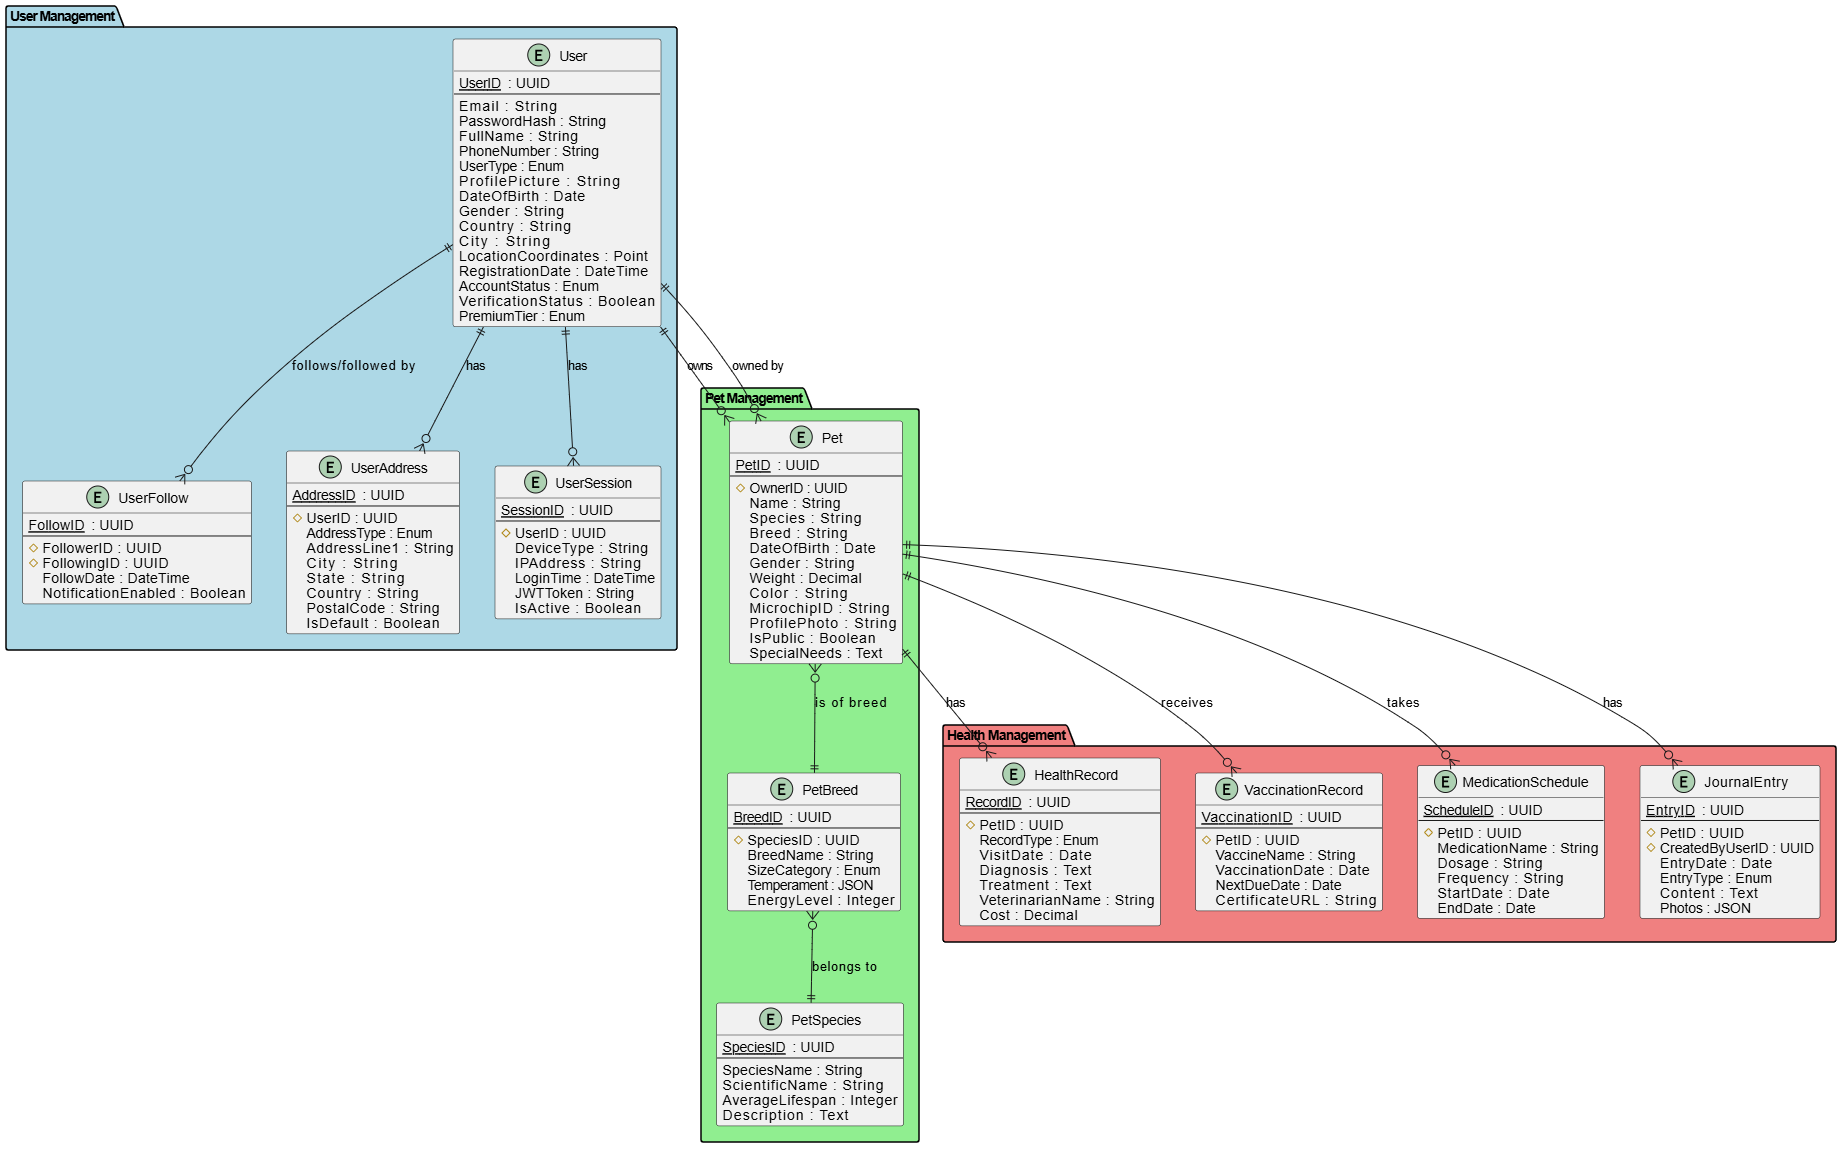
\includegraphics[width=\textwidth]{ThesisFigs/domain_model_core.png}
\caption{PawPal Domain Model - Core Entities (User and Pet Management)}
\label{fig:domain_core}
\end{figure}

The core domain model encompasses comprehensive Pet Management with species and breed classification systems, document management for certificates and records, and rich media capabilities for photos and videos. The Health Management sub-module integrates seamlessly with pet profiles to provide complete medical history tracking including vaccinations, medications, symptom tracking, growth monitoring, allergy management, and dietary profiling. Advanced features include training programs with progress tracking, behavioral issue management, intelligent reminder systems, and insurance policy integration with claims processing.

\subsection{Marketplace Module Entities}

The marketplace module implements a comprehensive e-commerce platform for pet products and supplies. Figure \ref{fig:domain_marketplace} presents the complete marketplace ecosystem including products, categories, shopping cart, orders, reviews, sellers, and promotional features. The architecture supports multi-vendor selling with individual seller profiles, product variants, inventory management, and integrated payment processing. The coupon and promotion system enables flexible marketing campaigns while the review system ensures transparency and trust.

\begin{figure}[H]
\centering
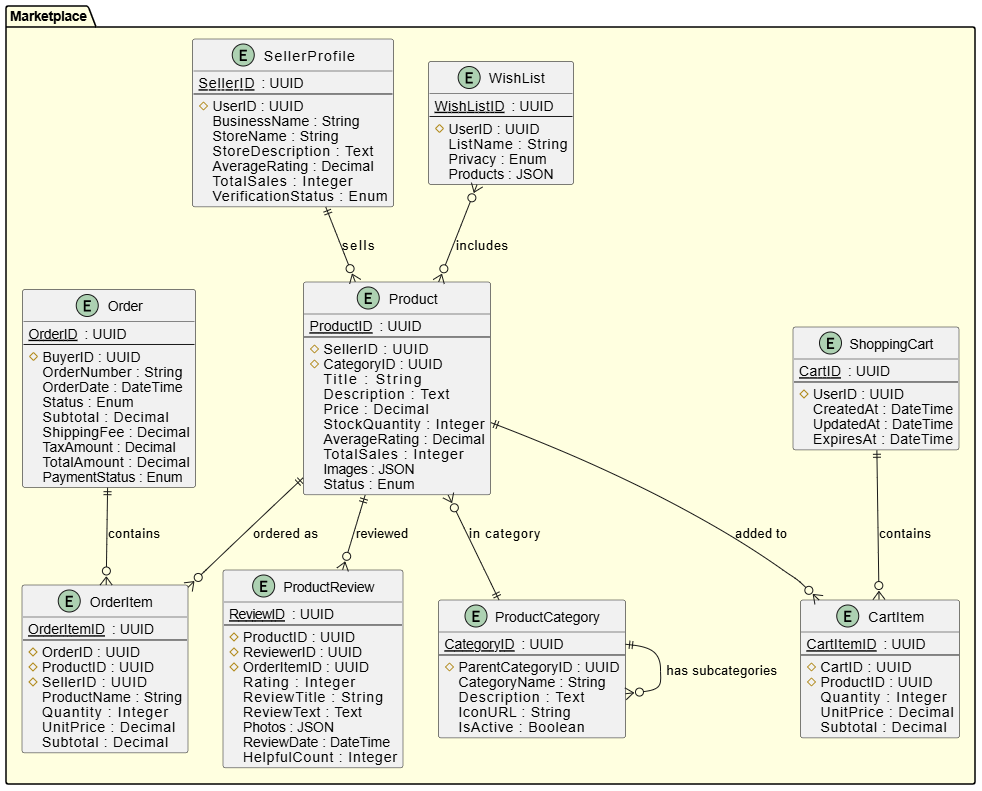
\includegraphics[width=\textwidth]{ThesisFigs/domain_model_marketplace.png}
\caption{PawPal Domain Model - Marketplace Module Entities}
\label{fig:domain_marketplace}
\end{figure}

Key marketplace entities include Product with 60+ attributes for pricing and inventory management, SellerProfile with business verification and performance metrics, Order entities for complete lifecycle tracking from cart to delivery, ProductReview for multi-dimensional ratings, ShoppingCart for session management, and Coupon/Promotion systems for marketing campaigns. The module supports product variants, wishlists, and comprehensive order status tracking with automated notifications.

\subsection{Community Hub Module Entities}

The community hub module fosters social interaction among pet owners through posts, groups, events, and specialized features. Figure \ref{fig:domain_community} illustrates the comprehensive social networking infrastructure including content creation, group management, event coordination, lost pet alerts, adoption listings, and engagement features. The module supports rich media sharing, real-time interactions, and community-driven content with moderation capabilities.

\begin{figure}[H]
\centering
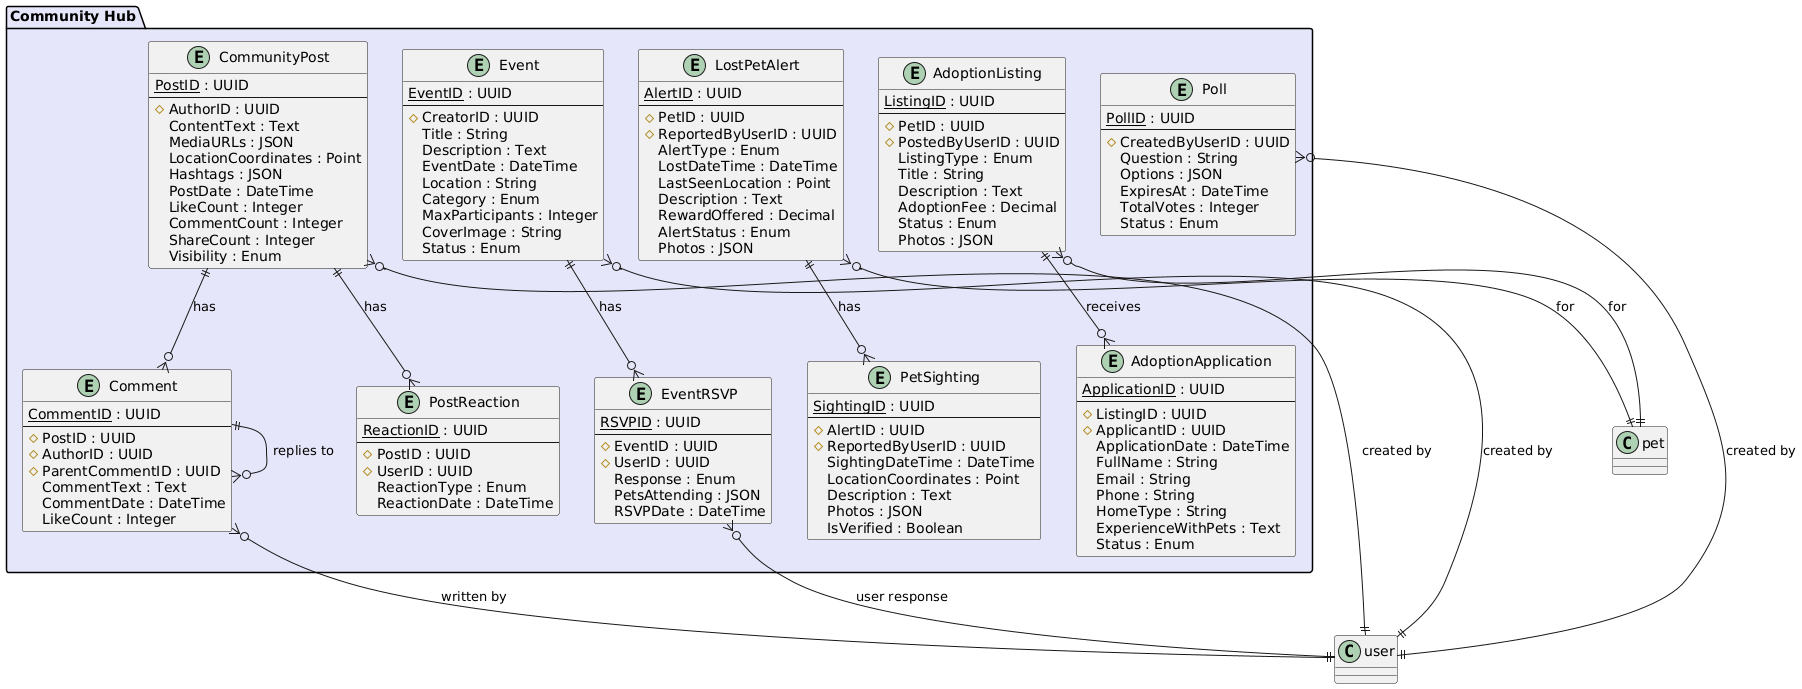
\includegraphics[width=\textwidth]{ThesisFigs/domain_model_community.png}
\caption{PawPal Domain Model - Community Hub Module Entities}
\label{fig:domain_community}
\end{figure}

The community module features CommunityPost entities for rich content with media and location tagging, Comment and PostReaction systems for engagement tracking, Group entities with role-based membership, Event management with RSVP capabilities, LostPetAlert with GPS tracking and PetSighting reports, AdoptionListing with application screening, StoryPost for temporary 24-hour content, and Poll entities for community feedback. The architecture supports hashtags, trending topics, and pet playdate coordination.

\subsection{Veterinary \& Caregiver Services Module Entities}

The services module connects pet owners with professional veterinary and caregiver services. Figure \ref{fig:domain_services} presents the service provider ecosystem including clinic management, appointments, online consultations, prescriptions, caregiver profiles, service bookings, and GPS-tracked service delivery. The module supports scheduling, reviews, certifications, and real-time service updates.

\begin{figure}[H]
\centering
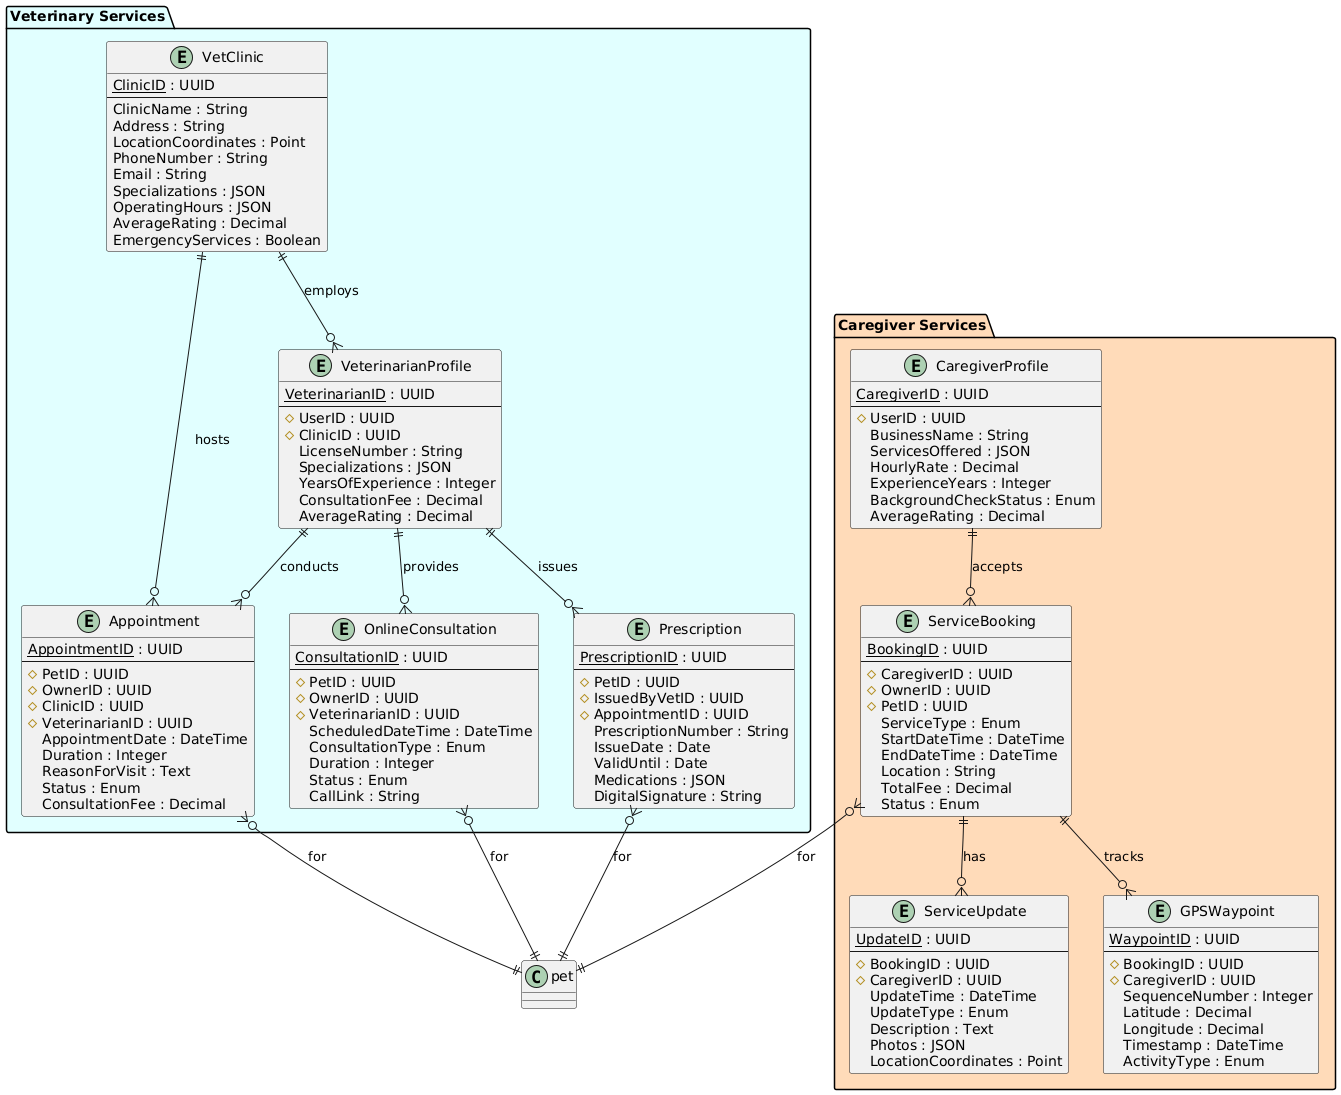
\includegraphics[width=\textwidth]{ThesisFigs/domain_model_services.png}
\caption{PawPal Domain Model - Veterinary \& Caregiver Services Module Entities}
\label{fig:domain_services}
\end{figure}

Key service entities include VetClinic with specializations and emergency services, VeterinarianProfile with certifications and experience tracking, Appointment scheduling with real-time availability, OnlineConsultation for video/audio/chat interactions, Prescription management with digital signatures, CaregiverProfile with background verification, ServiceBooking with status tracking, ServiceUpdate for photo/video proof of service completion, and GPSWaypoint for real-time location tracking during pet walks.

\subsection{Payment System \& AI Module Entities}

The payment and AI modules handle financial transactions and intelligent assistance. Figure \ref{fig:domain_payment_ai} illustrates the comprehensive payment infrastructure including traditional wallets, cryptocurrency support, invoicing, and dispute resolution, alongside AI-powered features for chatbot conversations, breed identification, and diet planning.

\begin{figure}[H]
\centering
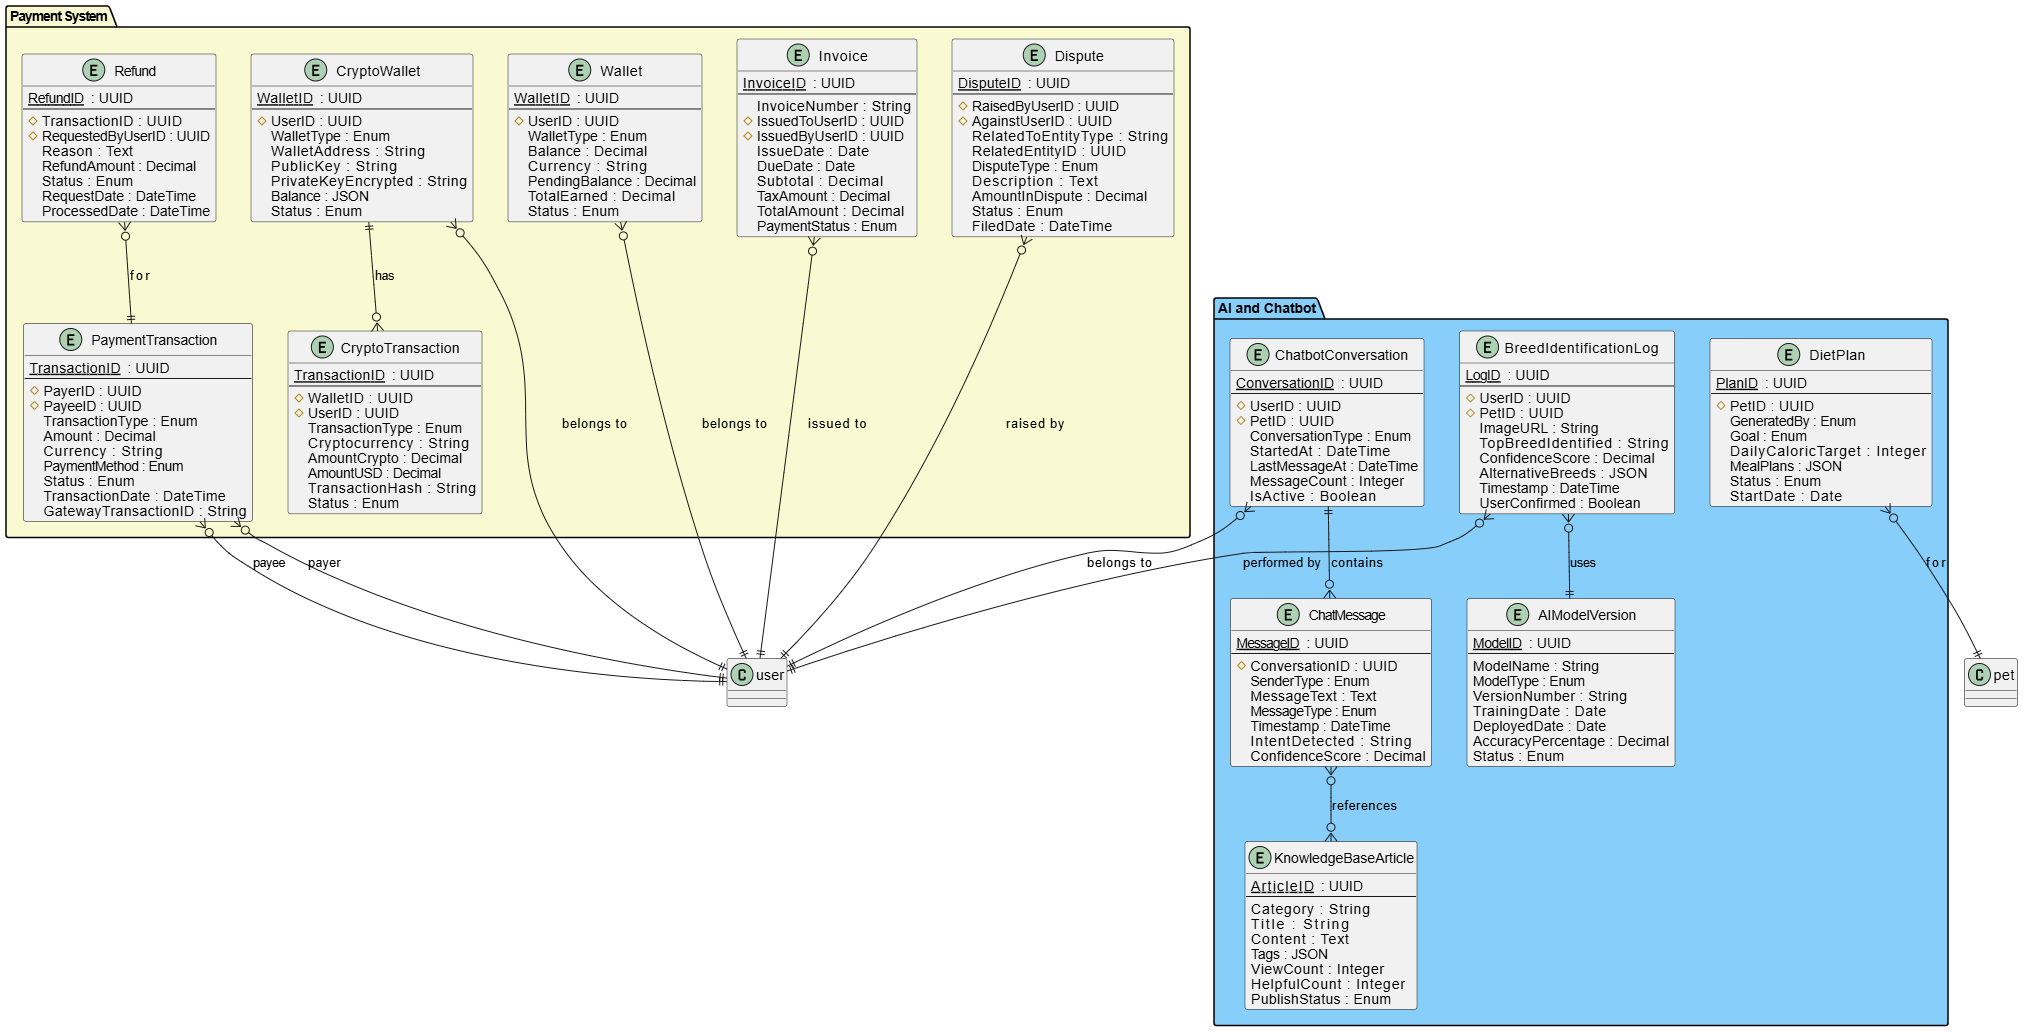
\includegraphics[width=\textwidth]{ThesisFigs/domain_model_payment_ai.png}
\caption{PawPal Domain Model - Payment System \& AI Module Entities}
\label{fig:domain_payment_ai}
\end{figure}

The payment system includes Wallet entities for multi-currency balance management, PaymentTransaction for comprehensive transaction logging, CryptoWallet supporting Bitcoin/Ethereum/USDT, CryptoTransaction, Invoice generation with itemization, Dispute resolution workflows, and Refund request management. The AI module features ChatbotConversation with intent detection, ChatMessage with confidence scoring, BreedIdentificationLog using CNN models, DietPlan with veterinary approval, AIModelVersion for performance tracking, and KnowledgeBaseArticle for medical information retrieval.

\subsection{Entity Relationships and Integration}

The comprehensive domain model establishes extensive relationships across all modules ensuring data integrity and supporting complex queries. Core relationships include User-Pet ownership (1:N), Pet-HealthRecord tracking (1:N), User-Order transactions (1:N), Product-Category classification (N:1), Post-Comment interactions (1:N hierarchical), User-Group membership (M:N), Appointment-HealthRecord generation (1:1), ServiceBooking-GPSWaypoint tracking (1:N), and PaymentTransaction-Order linkage (polymorphic N:1).

Cross-module integration enables users to participate across all modules in different roles (Owner/Seller/Vet/Caregiver/Admin), pets to be referenced in Health, Community, Vet Services, and Caregiver modules, payment transactions to connect Marketplace, Vet Services, and Caregiver modules, notifications to span all modules with user preferences, and reviews to exist for Products, Clinics, Veterinarians, and Caregivers. The model supports polymorphic relationships for extensibility while maintaining referential integrity through proper foreign key constraints and cascade rules.


